\documentclass[../main.tex]{subfiles}

\begin{document}
%%%%%%%%%%%%%%%%%%%%%%%%%%%%%%%%%%%%%%
%                                    %
% Integralrechnung IV -- Anwendungen %
%                                    %
%%%%%%%%%%%%%%%%%%%%%%%%%%%%%%%%%%%%%%
\chapter{SW11 Integralrechnung IV-- Anwendungen}
\section{Trapezregel}
Unterteile das Intervall $[a,b]$ in $n$ gleich grosse Teilintervalle $[x_{j-i},x_j],j=1,2,...,n$.\\
\begin{minipage}{0.45\textwidth}
    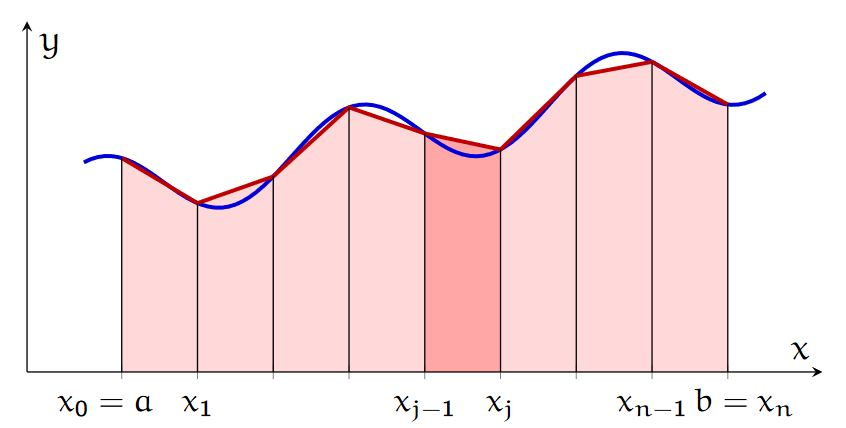
\includegraphics[width=50mm,scale=0.5]{trapezregel}
\end{minipage} \hfill
\begin{minipage}{0.5\textwidth}
    In jedem Teilintervall approximiere man die Funktion f durch eine lineare Funktion. \\
    Das Integral über jedes Teilintervall wird approximiert durch die Trapezfläche. 
\end{minipage}
Die Summe der Trapezflächen ist dann eine gute Approximation des bestimmten Integrals, vor allem wenn man $n$ genügend gross wählt: \\
$\int\limits_a^bf(x)dx\approx\sum\limits_{j=1}^n\frac{h}{2}(f(x_{j-1}+f(x_j))$ wobei $h=\frac{b-a}{n}$. \\
Der bei der Trapezregel \\
$\int\limits_a^bf(x)dx\approx\frac{b-a}{2}(f(x_0)+2f(x_1)+2f(x_2)+...+2f(x_{n-1})+2f(x_n)) = I_T(h)$ \\
gemachte Fehler $\epsilon_T$ ist für genügend anständige (zB stückweise stetige) Funktion $f$ beschränkt durch \\
$|\epsilon_T|=|\int\limits_a^bf(x)dx-I_T(h)|\leq\frac{(b-a)^3}{12n^2}max_{a\leq\epsilon\leq b} |f''(\epsilon)|$

\section{Trapezregel - kurz}
Funktion: $f(x)$ \\
Intervall: $[a,b]$ \\
Anzahl Teilintervalle: $n$ \\
\\
Fläche: $\int\limits_a^bf(x)dx=\frac{1}{2}\frac{b-a}{n}(y_0+2y_1+2y_2+...+2y_{n-1}+y_n)$ \\
$y_i$ also die versch. $y$ in Formel oben: $y_i=f(x_i)=f(a+i\frac{b-a}{n});0\leq i\leq n$

\subsection{Beispiel}
$f(x)=\frac{3}{x}$ \\
$[a,b]=[1,4]$ \\
$n=3$ \\
\\
$\int\limits_a^bf(x)dx=\frac{1}{2}\frac{b-a}{n}(y_0+2y_1+2y_2+...+2y_{n-1}+y_n)$
$=\frac{1}{2}\frac{4-1}{3}(y_0+2y_1+2y_2+y_3)$ \\
Die versch. $y$ herausfinden mit: $y_i=f(x_i)=f(a+i\frac{b-a}{n})$ \\
$y_0=f(x_0)=f(1+0\frac{4-1}{3})=f(1)=3$ \\
$y_1=f(x_1)=f(1+1\frac{4-1}{3})=f(2)=1.5$ \\
$y_2=f(x_2)=f(1+2\frac{4-1}{3})=f(3)=1$ \\
$y_3=f(x_3)=f(1+3\frac{4-1}{3})=f(4)=0.75$ \\
\\
Einsetzen: \\
$\frac{1}{2}\frac{4-1}{3}(3+2(1.5)+2(1)+0.75) = 4.375$ 

\section{Simpsonregel - kurz}
Funktion: $f(x)$ \\
Intervall: $[a,b]$ \\
Anzahl Teilintervalle: $n$ \\
\\
Fläche: $\int\limits_a^bf(x)dx\approx\frac{b-a}{6n}(y_0+4y_1+2y_2+4y_3+...+2y_{2n-2}+4y_{2n-1}+y_{2n})$ \\
$y_i$ also die versch. $y$ in Formel oben: $y_i=f(x_i)=f(a+i\frac{b-a}{2n});0\leq i\leq 2n$

\subsection{Beispiel}
Gleiches Vorgehen wie bei der Trapezregel!

\section{Definition Bogenlänge}
Ist $y=f(x)$ eine glatte Kurve ($f'$ ist stetig) im Intevall $[a,b]$, dann 
ist die Länge dieser Kurve über $[a,b]$ gegeben durch: \\
$L=\int\limits_a^b\sqrt[]{1+[f'(x)]^2}dx=\int\limits_a^b\sqrt[]{1+(\frac{dy}{dx})^2}dx$

\subsection{Beispiel}
Berechne die Bogenlänge $L$ der Kurve $y=x^{\frac{3}{2}}$ von $(1,1)$ nach $(2,2\sqrt[]{2})$. \\ [7pt]
$L=\int\limits_1^2\sqrt[]{1+(f'(x))^2}dx = \int\limits_1^2\sqrt[]{1+(\frac{3}{2})^2x^{(\frac{1}{2})^2}}dx$
$=\int\limits_1^2\sqrt[]{1+\frac{9}{4}x}dx$ \\ [7pt]
$t=1+\frac{9}{4}x$ \\ [7pt]
$dt=\frac{9}{4}dx$ \\ [7pt]
$dx=\frac{9}{4}dt$ \\ [7pt]
$=\int\limits_{\frac{13}{4}}^{\frac{22}{4}}\sqrt[]{t}\frac{4}{9}dt$
$=\int\limits_{\frac{13}{4}}^{\frac{22}{4}}t^{\frac{1}{2}}\frac{4}{9}dt$ \\ [7pt]
$\int t^{\frac{1}{2}}dt=\frac{t\frac{3}{2}}{\frac{3}{2}}$ \\ [7pt]
$=\frac{4}{9}\left[\frac{2}{3}t^{\frac{3}{2}}\right]_{\frac{13}{4}}^{\frac{22}{4}}$
$=\frac{8}{27}((\frac{22}{4})^{\frac{3}{2}}-(\frac{13}{4})^{\frac{3}{2}})$
$=\frac{8}{27(8)}(22\times\sqrt[]{22}-13\times\sqrt[]{13})$

\section{Kurven in Polarform}
Das Bogenelement ist \\
$(ds)^2=(rd\phi)^2+(dr)^2 = \sqrt[]{(r(\phi))^2+(r'(\phi))^2}d\phi$ \\
Integration von $\alpha$ bis $\beta$ liefert die Bogenlänge. \\
Die Bogenlänge einer in Polarkoordinaten gegebenen glatten Kurven (dh $r'$ stetig)
$r=r(\phi)$ mit $\alpha \leq \phi \leq \beta$ ist gegeben durch: \\
$L=\int\limits_\alpha^\beta\sqrt[]{(r(\phi))^2+(r'(\phi))^2}d\phi$

\subsection{Beispiel}
Man hat $r(\phi)=R$ und damit, weil $r$ gar nicht von $\phi$ abhängt $r'(\phi)=0$.
Also findet man für den Umfang des Kreises mit Radius $R$: \\
$U=\int\limits_0^{2\pi}\sqrt[]{(r(\phi))^2+(r'(\phi))^2}d\phi$
$=\int\limits_0^{2\pi}\sqrt[]{R^2+0^2}d\phi = \int\limits_0^{2\pi}Rd\phi = 2\pi R$

\section{Kurven in Parameterform}
Das infinitesimale Bogenelement der Kuve in Parameterform \\
$\gamma:[a,b]\to\mathbb{R}^2,t\mapsto \vec{x}(t)=
\begin{pmatrix}
    x(t) \\
    y(t)
\end{pmatrix}$ \\ [7pt]
ist gegeben durch \\ [7pt]
$ds=|\dot{\vec{x}}(t)|dt=\sqrt[]{(\dot{x}(t))^2+(\dot{y}(t))^2}dt$ \\ [7pt]
Integration von $t=a$ bis $t=b$ liefert die Bogenlänge der in Parameterform gegebene Kurve \\ [7pt]
$L=\int\limits_a^bds = \int\limits_a^b|\dot{\vec{x}}(t)|dt$
$=\sqrt[]{(\dot{x}(t))^2+(\dot{y}(t))^2}dt$ 

\section{Beispiel}
$\gamma=\begin{pmatrix}R\cos(t) \\R\sin(t)\end{pmatrix}$
$=R\begin{pmatrix}\cos(t) \\\sin(t)\end{pmatrix}$ \\ [7pt]
$\dot{\gamma}(t)=R\begin{pmatrix}-\sin(t) \\\cos(t)\end{pmatrix}$
$\begin{pmatrix}x(t) \\y(t) \end{pmatrix} $ \\ [7pt]
$(\dot{x}(t))^2=(-R\sin(t))^2=R^2\sin^2t$ \\ [7pt]
$(\dot{y}(t))^2=(R\cos(t))^2=R^2\cos^2t$ \\ [7pt]
$(\dot{x}(t))^2+(\dot{y}(t))^2=R^2\sin^2t+R^2\cos^2t=R^2(\sin^2t+\cos^2t)=R^2$ \\ [7pt]
$L=\int\limits_\alpha^\beta\sqrt[]{(\dot{x}(t))^2+(\dot{y}(t))^2}dt$
$=\int\limits_0^{2\pi}\sqrt[]{R^2}dt=\int\limits_0^{2\pi}Rdt=...=2\pi R$


\end{document}